\documentclass[11pt,a4paper,article]{memoir} 

\usepackage[T1]{fontenc}
\usepackage[utf8]{inputenc}
\usepackage[english, portuguese]{babel}

\usepackage{hyperref}
\usepackage{microtype}
\usepackage{acronym}
\usepackage{xstring}
\usepackage{minted-devel}
\usepackage{graphicx}
\usepackage{csquotes}
\usepackage[backend=bibtex, style=ieee]{biblatex}

\bibliography{bibliography.bib}

\newcommand{\foreign}[2][nohyphenation]{\protect\foreignlanguage{#1}{\slshape{#2}}}
\newcommand{\english}[1]{\foreign[english]{#1}}

% Typeset Programming Code
\newcommand{\code}[1]{\texttt{\textbf{#1}}}
\newenvironment{displaycode}
  {%
    \begin{flushleft}%
    \ttfamily%
    \begin{tabbing}%
    1234567890\=12345678\=12345678\=12345678\=12345678\=12345678\=\kill%
  }
  {%
    \end{tabbing}%
    \end{flushleft}%
  }


% Exercicio

\newcounter{Exctr}
\newenvironment{exercicio}%
{%
\refstepcounter{Exctr}%
\noindent\begin{minipage}{\textwidth}
\vspace*{5pt}
\noindent%
\makebox[0pt]{\rule[-4pt]{1pt}{5pt}}%
\rule{1.05\textwidth}{1pt}%
\makebox[0pt]{\rule[-4pt]{1pt}{5pt}}%
\\
\hspace*{6pt}\textbf{\large Exercício \arabic{chapter}.\arabic{Exctr}}\vspace*{10pt}\\
\hspace*{0.025\textwidth}\begin{minipage}[t]{0.95\textwidth}
}%
{%
\end{minipage}
\hfill\\
\noindent\makebox[0pt]{\rule{1pt}{5pt}}%
\rule{1.05\textwidth}{1pt}%
\makebox[0pt]{\rule{1pt}{5pt}}
\vspace*{5pt}
\end{minipage}\\
}


% Short defs
\def\linux{\english{Linux}}


\normalsize
\def\b{\textbackslash}
\def\bibtex{BibTeX}

\newcommand{\single}[1]{
'#1'
}

\newcommand{\herebox}{\vspace{3mm}\fbox{\textbf{\texttt{\result}}}\vspace{3mm}}

\newcommand{\showresult}{
\vspace{3mm}
\fbox{\textbf{\result}} $\rightarrow$ \tokenize{\resultx}{\result} \resultx
\vspace{3mm}

}

\newcommand{\showresultm}{
\vspace{3mm}
\fbox{\textbf{\result}} $\rightarrow$ \tokenize{\resultx}{\result} $\resultx$
\vspace{3mm}

}

\newcommand{\showresultc}[1]{
\vspace{3mm}
\fbox{\textbf{\result}} $\rightarrow$ #1
\vspace{3mm}

}

\newcommand{\showresultcc}[1]{
\vspace{3mm}
\fbox{\textbf{\result}} $\rightarrow$ \tokenize{\resultx}{\result} {\resultx} #1
\vspace{3mm}

}

\newcommand{\exemplofile}[2]{
\vspace{5mm}
\small
\begin{center}
\begin{minipage}{10cm}
\inputminted{latex}{#1}
\end{minipage}
\vspace{5mm}\\
\huge$\Downarrow$\small\\
\vspace{5mm}
\begin{minipage}{10cm}
\input{#1}
\end{minipage}
\vspace{5mm}
\end{center}
}

\pretitle{\begin{center}\Huge\bfseries}
\title{Introdução ao \LaTeX}
\posttitle{\par\vskip1em{\normalfont\normalsize\scshape Departamento de Electrónica, Telecomunicações e Informática\\Universidade de Aveiro\\%
\vspace{20mm}
\includegraphics{latex-intro/ua.pdf}\par\vfill}\end{center}}

\author{André Zúquete, João Paulo Barraca, Diogo Gomes}
\predate{\vfill\begin{center}v1.0, \large}
\date{Setembro de 2014}
\postdate{\end{center}}

\begin{document}

\maketitle

\newpage
\tableofcontents*
\newpage
\listoffigures*
\newpage

\chapter{Introdução}

O {\LaTeX} é uma ferramenta de apoio à produção de documentos
complexos (particularmente de índole técnica). O seu paradigma de funcionamento é completamente
diferente do de outras ferramentas mais populares atualmente, como o
\english{Word} da \english{Microsoft}. Enquanto editores tradicionais, 
denominados \ac{wysiwyg} focam-se na construção simultânea de todo
o documento, incluindo aspeto gráfico e conteúdo, o {\LaTeX} assume que
o autor se deve focar no conteúdo, categorizando apenas o texto produzido,
sem se preocupar imediatamente com o aspeto. Este tipo de sistemas são
denominados por \ac{wysiwym}.

Portanto, ao escrever um documento utilizando {\LaTeX}, devemos focar-nos
em adicionar conteúdo e em especificar o que queremos como título, secção,
tabela, ou que imagens queremos incluir. Aspetos como o estilo, tipo de letra,
localização das imagens, espaçamentos, paginação e mesmo hifenação
ficam a cargo do {\LaTeX}. O autor pode refinar estes pontos, mas à partida não terá
de se preocupar com eles. Para mais informação sobre customização, pode consultar
\cite{wikibooks-latex}\cite{tex-stackexchange}.

O {\LaTeX} é a ferramenta por excelência para a realização de relatórios
de caráter técnico, publicações científicas e mesmo guiões para
aulas. Neste documento iremos descrever os
conceitos elementares para produzir um documento minimamente estruturado em 
{\LaTeX}.


%
%
% SECCAO : Compilação
%
%
\chapter{Compilação de documentos {\LaTeX}}

Os documentos {\LaTeX} são produzidos editando ficheiros de texto
com um editor elementar, como o \code{vim}. Esta aproximação facilita
a edição colaborativa pois reduz aspetos de compatibilidade entre sistemas.
Qualquer editor de texto pode ser utilizado, o que permite que um documento seja
facilmente editado. Este mesmo documento foi parcialmente realizado em 
sistemas \english{Windows}, \english{OS X} e {\linux}.

Os ficheiros {\LaTeX} são então facilmente alterados por humanos, contendo o
texto que deverá constar do documento final a produzir, juntamente com comandos
relativas à sua formatação.

De notar que ao editar um documento através do sistema {\LaTeX}, não estaremos a ver
como o documento realmente irá ser apresentado. Para isso é necessário um passo de
compilação. Esta compilação converte o documento {\LaTeX} para um outro formato,
sendo que o mais utilizado é o \ac{pdf}. Pode considerar que o conceito é semelhante
ao da compilação de um programa \english{Java} no formato \code{.java} 
para um ficheiro \code{.class}.

Existem editores especializados que permitem ter uma vista quase em tempo real do
documento final. Na realidade, estes editores estão constantemente a compilar 
o documento, apresentando depois o resultado ao utilizador. 
Um exemplo é o \code{gummi}, outro o \code{texmaker}, mas existem ainda muitos 
outros\footnote{Veja \url{http://tex.stackexchange.com/questions/339/latex-editors-ides}}.

Para compilar um documento {\LaTeX} é necessário executar o compilador, seguido do
ficheiro a compilar. Por exemplo, assumindo que o nosso ficheiro se chama 
\code{hello.tex}, poderemos compilar o ficheiro para \ac{pdf} através 
do comando:\\

\code{\$ pdflatex hello.tex}\\

\noindent
O resultado deverá ser um conjunto de ficheiros auxiliares (que podem ser removidos), e
um documento com extensão \ac{pdf}. Na \autoref{diagram} voltaremos a este assunto.

\begin{exercicio}
No sítio da disciplina existe um ficheiro chamado \code{hello.tex}. Obtenha este 
ficheiro. O conteúdo deste ficheiro ainda não é relevante. Compile este ficheiro
 e verifique que é produzido um ficheiro com extensão \acs{pdf}.\\

Verifique que consegue visualizar o conteúdo do ficheiro {\LaTeX} utilizando o comando
\code{vim}.\\

Pode igualmente editar o ficheiro através da aplicação \code{texmaker}. A vantagem
desta aplicação é já ter algumas funcionalidades que auxiliam a produção de
documentos {\LaTeX}.\\

Para visualizar o documento produzido, pode utilizar as aplicações \code{epdfview} 
ou \code{evince}.
\end{exercicio}


%
%
%
% ESTRUTURA DE UM DOCUMENTO
%
%
%
\chapter{Estrutura obrigatória de um documento}
\label{sec.class}

A estrutura obrigatória de um documento passa em primeiro lugar, e
obrigatoriamente, pela definição do seu tipo de estrutura, pela
definição do tipo de letra base (tipo e caixa), pela definição do
dimensão da página, pela definição da estrutura da mancha na página
(uma coluna, duas colunas), etc.

Esta estrutura é definida pelo comando \verb|\documentclass[options]{class}|.
O seu parâmetro obrigatório é a classe de documento, a qual define o
tipo base de documento. Eis alguns exemplos de classes: \code{book},
\code{report}, \code{article}.  Os parâmetros opcionais podem ser
(lista não exaustiva):
\begin{description}
\item[\code{a4paper}, \code{a5paper}, etc.]: dimensão da folha.
\item[\code{10pt}, \code{11pt}, \code{12pt}]: dimensão caixa da letra base.
\item[\code{onecolumn} ou \code{twocolumn}]: texto com uma ou duas colunas.
\item[\code{oneside} ou \code{twoside}]: só frente ou frente e verso.
\end{description}
\noindent
Este é um exemplo para especificar um relatório em páginas a4, com
caixa base de 11pt, a duas colunas e frente-e-verso:

\verbtocs{\result}|\documentclass[a4paper,11pt,twocolumn,twoside]{report}|{\herebox}

\noindent
Após esta especificação, o conteúdo efetivo do documento deverá ser
colocado entre dois comandos: \verb|\begin{document}|
e \verb|\end{document}|.\\

\begin{minted}{latex}
\documentclass[a4paper]{article}

\begin{document}

% conteúdo do documento

\end{document}
\end{minted}

\begin{exercicio}
Copie o documento \code{hello.tex} para um novo ficheiro e produza o \ac{pdf}
respetivo. Altere as suas opções e coloque novas opções, observe o
resultado. Coloque muito mais conteúdo, de forma a produzir
múltiplas páginas, altere novamente as opções, e observe o resultado.
\end{exercicio}

%
%
% SECCAO: CARACTERES ESPECIAIS
%
%
%
\chapter{Caracteres especiais do {\LaTeX}}
\label{specials}

No ficheiro que já compilou pode verificar que, além do texto, existem diversas 
instruções, que denominámos por comandos. Estes usam caracteres que
normalmente não fazem parte do conteúdo de um texto de um documento,
a saber: {\b},\{, \}, [, ], \$, \%, \~{ }, \#, \_,
\textasciicircum, e \&. Neste momento é prematuro introduzir o
significado de todos eles, vamos apenas apresentar alguns já de seguida.

\section{O caráter \single{\b}}

O caráter \single{\b} é o símbolo base da definição de comandos, daí que
normalmente está no seu início:

\verbtocs{\result}|\o| \showresult 
\verbtocs{\result}|\oe| \showresult 
\verbtocs{\result}|\LaTeX| \showresult 

\noindent
Para escrever o caráter \single{\b} num texto (o que é raro) é preciso recorrer a um
comando:

\verbtocs{\result}|\textbackslash| \showresult

\begin{exercicio}
Edite o documento e adicione estes comandos 
depois do texto ``Hello World!''. Não se esqueça de compilar o 
documento e verificar o resultado! 
\end{exercicio}


\section{O caráter \single{\$}}

O caráter \single{\$} é usado para sinalizar a entrada e saída do
modo matemático. Por omissão o conteúdo fonte de um documento
{\LaTeX} é interpretado em modo de texto, entrando no modo
matemático é saindo do mesmo com este caráter. O modo matemático
será abordado mais adiante.

\verbtocs{\result}|text mode, $math mode$, text mode| \showresult

\noindent
Para escrever o caráter \single{\$} num texto é preciso recorrer a um comando:

\verbtocs{\result}|\$| \showresult


\section{Os carateres \single{\{} e \single{\}}}

Estes caracteres, chavetas, servem para dois fins: definir um contexto e
definir um parâmetro de um comando.

Um contexto consiste num bloco de texto, entre as duas chavetas (a
de abrir e a de fechar), que delimita o universo de abrangência de
comandos de formatação expressos nesse mesmo bloco. Ou seja, uma
formação imposta dentro de um bloco não tem efeito fora do bloco.
Neste âmbito, as chavetas servem também para delimitar corretamente
os comandos que não possuem parâmetros, nomeadamente para não usarem
o espaço que após os mesmos como terminador.

\verbtocs{\result}|\o e| \showresultcc{(o espaço é interpretado como terminador de \single{\b o})}
\verbtocs{\result}|{\o} e| \showresultcc{(o espaço é preservado como separador de \single{\b o} e \single{e})}

\noindent
Quando os comandos possuem parâmetros obrigatórios, estes são
normalmente indicados entre chavetas (alguns necessitam de estar delimitados por \$) :

\verbtocs{\result}|\acute{a}| \showresultm
\verbtocs{\result}|\vec{x}| \showresultm
\verbtocs{\result}|\sqrt{x}| \showresultm
\verbtocs{\result}|\textsc{texto em Small Caps}| \showresult
\verbtocs{\result}|\fbox{texto emoldurado}| \showresult
\verbtocs{\result}|\footnote{Nota de rodap\'e}| \showresult

\noindent
Quando os comandos possuem mais do que um parâmetro, cada um dos
parâmetros é indicado entre chavetas:

\verbtocs{\result}|\frac{x}{y}| \showresultm

\noindent
Para escrever os carateres \single{\{} ou \single{\}} num texto (o
que é raro) é preciso recorrer a um comando:

\verbtocs{\result}|\{ \}| \showresult

\begin{exercicio}
Edite o documento e adicione alguns destes comandos junto do restante texto.\\

Pode igualmente experimentar outras formatações de texto como \textbf{negrito}
(\verb|\textbf{negrito}|), ou \textit{itálico} (\verb|\textit{itálico}|).

\end{exercicio}


\section{Os carateres \single{[} e \single{]}}

Este carateres normalmente são interpretados literalmente (i.e.,
sem qualquer significado especial) exceto quando delimitam opções de
comandos:

\verbtocs{\result}|\sqrt[3]{x}| \showresultm

\section{O caráter \single{\%}}

O caráter \single{\%} é usado para sinalizar o início de texto que
não deverá ser interpretado, até ao final da linha corrente.

\verbtocs{\result}|texto interpretado, %texto ignorado| \showresultc{texto interpretado,}

\noindent
Para escrever o caráter \single{\%} num texto é preciso recorrer a um comando:

\verbtocs{\result}|\%| \showresult

\section{O caráter \single{\textasciitilde}}

O caráter \single{\textasciitilde} é usado para representar um
espaço entre dois elementos que nunca devem ficar separados em duas
linhas consecutivas. Por exemplo, quando se escreve ``\emph{a arquitetura apresentada na
figura 5}'' não é correto que ocorra uma translineação entre
``\emph{figura}'' e ``\emph{5}'', porque isso prejudica a leitura do
texto. Para sinalizar esse facto, escreve-se:

\verbtocs{\result}|a arquitetura apresentada na figura~5| \showresult

\noindent
Para realmente escrever o caráter \single{\textasciitilde} num texto é preciso
recorrer a um comando:

\verbtocs{\result}|\textasciitilde| \showresult



%
%
%
% FUNCIONALIDADES ADICIONAIS
%
%
%

\chapter{Funcionalidades adicionais}

Normalmente nos documentos {\LaTeX} usam-se funcionalidades para
além das incluídas da especificação base da ferramenta. Essas
funcionalidades são disponibilizadas em pacotes
(\english{packages}), os quais são normalmente indicados no início
de um documento através do comando
\verb|\usepackage[options]{packages}[version]|.
É também comum usar um comando destes por cada pacote usado.

Um exemplo de pacote que lhe poderá ser útil é o que permite
interpretar corretamente carateres para além dos contemplados na
tabela \ac{ascii}\footnote{Também pode consultar: \url{http://en.wikipedia.org/wiki/ascii}}, de
que são exemplo todos os caracteres latinos acentuados e os
caracteres de outros alfabetos que não o latino (grego, cirílico,
árabe, etc.). Este pacote é o \code{inputenc}, que tem como opção a
escolha do modo como os caracteres não \ac{ascii} estão codificados no
document fonte:

\verbtocs{\result}|\usepackage[encoding name]{inputenc}|{\herebox}

\noindent
Este documento, por exemplo, foi escrito em {\LaTeX} com codificação
utf8\footnote{utf8 é uma codificação que pretende ser uniforme para todas as
línguas.}, o que implicou a inclusão deste pacote do seguinte modo:

\verbtocs{\result}|\usepackage[utf8]{inputenc}|{\herebox}

\begin{exercicio}
Observe o resultado do \ac{pdf} obtido quando se usa ou não o pacote (experimente comentar a
linha da sua inclusão).
\end{exercicio}

Outro pacote que é útil para português é o \code{babel}, que ensina o {\LaTeX} a
realizar corretamente a translineação de palavras:

\verbtocs{\result}|\usepackage[languages]{babel}|{\herebox}

\noindent
Caso um documento inclua textos de várias línguas, como português e
inglês, tal é suportado pelo pacote:

\verbtocs{\result}|\usepackage[portuguese,english]{babel}|{\herebox}

Finalmente, outro pacote que é útil para português é o
\code{fontenc}, que indica o tipo de codificação de caracteres do
resultado da compilação do {\LaTeX}.  Aconselha-se o uso da
codificação \verb|T1|, porque a mesma permite lidar convenientemente com
caracteres acentuados.

\verbtocs{\result}|\usepackage[T1]{fontenc}|{\herebox}

\begin{exercicio}
Crie um novo ficheiro contendo texto em português e em inglês. Cada parágrafo deverá
ocupar mais do que uma linha de texto e deverá ter uma palavra translineada.\\

Verifique que o {\LaTeX} procede à translineação automática do texto apresentado. No
entanto esta poderá não ser a mais adequada à linguagem em causa.\\

O comando \verb|\selectlanguage{languagename}| permite especificar qual a língua do texto que se lhe segue. Use-o.
\end{exercicio}

%
%
% Dimensão das letras
%
%
%
%
%
\chapter{Dimensão das letras}

A dimensão base das letras é definida com o comando
\verb|\documentclass|, como vimos na \autoref{sec.class}. Este tamanho é
indicado com o comando \verb|\normalsize|. relativamente a este
tamanho o {\LaTeX} possui outras dimensões, a saber:\\

\label{sizes}
\centerline{
\begin{tabular}{ll}\hline
\textbf{Comando}    &  \textbf{Resultado para este documento} \\ \hline\hline
{\normalsize\texttt \b tiny} &  {\tiny texto de exemplo}        \\
{\normalsize\texttt \b scriptsize}       &  {\scriptsize texto de exemplo}  \\
{\normalsize\texttt \b footnotesize}    &  {\footnotesize texto de exemplo}\\
{\normalsize\texttt \b small}           &  {\small texto de exemplo}       \\
{\normalsize\texttt \b normalsize}      &  {\normalsize texto de exemplo}  \\
{\normalsize\texttt \b large}           &  {\large texto de exemplo}       \\
{\normalsize\texttt \b Large}           &  {\Large texto de exemplo}       \\
{\normalsize\texttt \b LARGE}        	&  {\LARGE texto de exemplo}       \\
{\normalsize\texttt \b huge}        	&  {\huge texto de exemplo}        \\
{\normalsize\texttt \b Huge}        	&  {\HUGE texto de exemplo}        \\ \hline
\end{tabular}\\
}

\exemplofile{latex-intro/tamanhos}{\small}

Como pode reparar, quando se escreve um documento, não existe a necessidade de ajustar
o tamanho das letras para valores específicos. 
Apenas se indica o que se pretende que seja maior ou menor, com base na referência
do documento. Desta forma ele ficará sempre coerente.

%
%
%
% ESTRUTURACAO DE UM DOCUMENTO
%
%
%
\chapter{Elementos estruturais de documentos}

\section{Título}

Nos documentos com título o mesmo é criado com recurso aos seguintes
comandos:
\begin{description}
\item\verb|\title{título}|: Define o texto do título. Se o mesmo
     tiver de ser dividido por várias linhas deverá ser usado o
     comando \verb|\\| para mudar de linha.
\item\verb|\author{autores}|: Define os autores. Também neste caso os
     autores podem ser divididos por várias linhas usado o comando
     \verb|\\| para mudar de linha. Nesta parte podem ainda ser
     incluídos outros atributos relativos aos autores para além do
     seu nome, como afiliações, endereços, etc.
\item\verb|\date{data}|: Define a data de criação do documento, que
     é apresentada no título. O comando \verb|\today| fornece a data atual.
     Para não incluir data deve-se usar uma data vazia (ou seja,
     nada entre as chavetas).
\item\verb|\maketitle|: Cria o título de acordo com o texto do
     mesmo, os autores e a data antes definidos.
\end{description}

Convem que estes documentos existam no início do documento, tal como acontece
no ficheiro \code{hello.tex}.\\

\section{Partes, capítulos, secções e parágrafos}

Os documentos podem ser seccionados com os seguintes comandos, cujo
nome é sugestivo:

\begin{description}
\item\verb|\part{title}|: inicia uma parte de documento (pode englobar vários
capítulos);
\item\verb|\chapter{title}|: inicia um capítulo (pode englobar vários secções);
\item\verb|\chapter{title}|: inicia uma secção (pode englobar vários subsecções);
\item\verb|\section{title}|: inicia uma subsecção (pode englobar vários sub-
subsecções);
\item\verb|\subsection{title}|: inicia uma sub-subsecção (pode englobar vários
parágrafos);
\item\verb|\paragraph{title}|: inicia um parágrafo (pode englobar vários
subparágrafos);
\item\verb|\subparagraph{title}|: inicia um sub-parágrafo.
\end{description}

\noindent
Todos estes comandos de seccionamento têm obrigatoriamente um
título, o qual terá a fonte e dimensão de caixa apropriadas
escolhidas automaticamente pelo {\LaTeX}. Eles são igualmente
numerados de forma automática e segundo estilos definidos pelo tipo
de documento (numeração romana ou árabe, letras, etc.).
Mais uma vez, ao utilizar {\LaTeX}, o autor especifica qual a função do texto,
deixando a composição gráfica a cargo do {\LaTeX}

\begin{exercicio}
Experimente usar todos estes comandos de seccionamento num
documento. Note que nem todos são possíveis em cada tipo de
documento (v.g. com documentos do tipo \code{article} não existe
\verb|\chapter|).
\end{exercicio}

\begin{exercicio}
Experimente incluir o comando \verb|\tableofcontents| logo no
início do texto útil do documento. Observe o resultado após compilar
o documento. Altere alguns dos títulos das secções, compile e
observe o resultado. Poderá ter de repetir a compilação para a criação correta
deste índice.
\end{exercicio}

Alguns dos títulos criados por estes comandos, como os de
\verb|\part|, \verb|\chapter| e \verb|\tableofcontents|, incluem
uma parte em inglês. Esta parte é automaticamente colocada pelo
{\LaTeX} de acordo com variáveis pré-definidas e com a língua definida,
as quais podes ser alteradas no documento com os seguintes comandos:\\


\begin{minted}{latex}
\renewcommand{\partname}{Parte}
\renewcommand{\chaptername}{Tema}
\renewcommand{\chaptername}{Secção}
\renewcommand{\contentsname}{Índice}
\end{minted}

\begin{exercicio}
Altere a ordem de declaração das línguas junto do pacote \code{babel}.
Volte a compilar a verifique qual o nome fornecido

Altere novamente o seu documento para incluir estas alterações
logo no início do texto útil do documento. Observe o resultado após compilar o
documento.
\end{exercicio}

%
%
%
%
%
\section{Listas de itens}

O {\LaTeX} inclui várias formas de listas de itens, tanto numeradas
como não numeradas. Estas listas são automaticamente indentadas pelo
{\LaTeX}.

Uma lista não numerada é criada através do ambiente \code{itemize}:
\exemplofile{latex-intro/itemize.tex}{\small}
\noindent
onde cada item é iniciado através do comando \verb|\item|. Em cada
comando \verb|\item| pode indicar um conteúdo alternativo para o
símbolo que o {\LaTeX} usa para iniciar o item (v.g.~\verb|\item[+]|
usa o símbolo \single{+}, ver abaixo):
\exemplofile{latex-intro/itemize.plus.tex}{\small}

Outra forma de criar uma lista não numerada é através do ambiente
\code{description}, onde cada item é iniciado por texto (ou título)
arbitrário em vez de um símbolo gráfico:
\exemplofile{latex-intro/description.tex}{\small}
\noindent
onde cada item é iniciado através do comando \verb|\item[title]|; o
parâmetro opcional (que pode ser omitido) é escrito em negrito.

As listas numeradas são criadas através do ambiente \code{enumerate}:
\exemplofile{latex-intro/enumerate.tex}{\small}
\noindent
onde cada item é iniciado através do comando \verb|\item| e
numerado automaticamente pelo {\LaTeX}. A numeração segue um formato
por omissão (v.g. numeração árabe) a qual pode ser mudada em cada
lista logo após a sua iniciação, como neste exemplo:
\exemplofile{latex-intro/enumerate.Roman.tex}{\small}
\noindent
onde cada item é numerado com numeração romana maiúscula; o termo
\code{enumi} representa o contador usado na listagem.
No exemplo abaixo mostra-se como se pode misturar vários tipos
de numeração:

\exemplofile{latex-intro/enumerate.Mix.tex}{\small}
\noindent

No primeiro nível usou-se numeração Romana maiúscula; no segundo nível
usaram-se letras minúsculas (começando em \single{a}).
\textbf{Nota}: a indentação usada neste último exemplo é irrelevante para o
{\LaTeX}, ela apenas facilita a compreensão do leitor.

%
%
%
%
\section{Objetos flutuantes: figuras e tabelas}

No {\LaTeX} existe um conceito, denominado de objetos flutuantes
(\english{floats}), que consiste na existência de objetos cujo lugar
não precisa de ser fixo, porque pode ser referenciado de outra forma
(v.g. através de um número de referência). Há dois tipos de objetos
flutuantes: figuras e tabelas.

As figuras e as tabelas são em tudo idênticas, exceto na maneira
como é apresentada a sua legenda. São objetos que podem conter
qualquer conteúdo (texto, imagens, etc.) e que possuem pelo menos
uma legenda. As legendas são numeradas e o seu número pode ser usado
noutros locais do texto para referir o objeto.

Uma figura é declarada do seguinte modo:\\

{\small
\inputminted{latex}{latex-intro/figure.tex}
}

\noindent
e o resultado é a figura abaixo:
\begin{figure}[h]
 \centerline{\fbox{Conteúdo da figura, pode ser texto, imagem, etc.}}
\caption{Legenda da figura}
\end{figure}


\noindent
A opção \single{h} indicada no início do ambiente \code{figure}
indica que a figura deverá primordialmente ser colocada no lugar
onde aparece em termos de fluxo de texto. Mas tal nem sempre é
possível. O {\LaTeX} possui heurísticas internas que determinam a melhor
localização de um objeto flutuante de forma a que o documento fique mais
equilibrado. O resultado é que os objectos flutuantes nem sempre irão ficar onde
são declarados de forma melhorar o aspeto final do documento.

Outras opções para além da \single{h} são:
\begin{description}
\item \code{t} - A figura é colocada no topo da página.
\item \code{b} - A figura é colocada no fundo da página.
\item \code{p} - A figura é colocada numa página isolada.
\end{description}
Várias destas opções podem ser usadas, indicando uma ordem de
preferência para o {\LaTeX}.

Tanto as figuras como as tabelas podem ser referidas através do seu
número. Em {\LaTeX} essa funcionalidade é obtida através dos
comandos \verb|\label| e \verb|\ref|. Se utilizar o \english{package}
\english{hyperref}, é possível também usar o comando \verb|\autoref|.
Estes comandos são descritos em maior pormenor na secção seguinte.

As tabelas seguem exatamente as mesmas regras que as figuras,
simplesmente usa-se o ambiente \code{table} e a legenda é
identificada de forma diferente. Assim, uma tabela é declarada do
seguinte modo:\\

{\small
\inputminted{latex}{latex-intro/table.tex}
}

\noindent
e o resultado é a tabela abaixo:
\begin{table}[htp]
\caption{Exemplo de uma tabela}
 \centerline{Conteúdo de uma tabela}
\label{etiqueta}
\end{table}%


Note-se que nesta tabela usou-se o comando \verb|\label| para a
referir neste texto pelo seu número (\autoref{etiqueta}, obtido através da 
etiqueta \code{etiqueta} no comando \verb|\autoref{etiqueta}|). 
Veja a secção seguinte para
obter mais pormenores sobre este tipo de comandos. Também nesta tabela
usou-se o comando \verb|\caption| antes do conteúdo da tabela, o que
causou que a legenda da tabela aparecesse no seu topo.

\begin{exercicio}
Edite o seu documento e coloque-lhe várias figuras e tabelas,
contendo uma ou mais figuras/tabelas por objeto flutuante.
Experimente as diversas colocações e veja o que acontece com cada
uma delas. Confirme também que os objetos flutuantes do mesmo tipo
(figuras ou tabelas) nunca ficam por uma ordem diferente daquela em
que são declaradas, muito embora possam ficar fora do local onde
forsam indicadas no documento fonte.
\end{exercicio}

%
% Referencias
%
%
\section{Referências a partes do texto}
\label{refs.Section}

Qualquer identificador numérico usado num documento {\LaTeX}, seja
ele de parte, capítulo, secção, lista numerada, figura, tabela, e
outros, pode ser usado no texto através dos comandos \verb|\label|
, \verb|\ref| e \verb|\autoref|.

O comando \verb|\label| associa uma etiqueta a um número usado
num dos elementos acima referidos (parte, capítulo, etc.). Para
isso, o normal é colocar a etiqueta imediatamente após o comando que
produz o número que se pretende, muito embora isso não seja
estritamente necessário. Por exemplo, o início desta secção foi
escrito com o seguinte conteúdo:\\

{\small
\inputminted{latex}{latex-intro/refs.tex}
}

\noindent
Assim, o comando \verb|\ref{refs.Section}| produzirá o número
\ref{refs.Section}. A vantagem deste método é que o texto pode ser
livremente alterado, inclusive alterada a sua ordem, que os números utilizados
para as imagens, figuras e as respetivas referências é mantido de forma ordenada.
Também pode ser usado o método \verb|\autoref{refs.Section}| que irá gerar uma
descrição mais longa: \autoref{refs.Section}.

O uso destes comandos obriga normalmente a duas compilações
de um documento para que os valores apresentados pelas referências
estejam corretos. Na primeira compilação é obtido e guardado o
número associado a cada etiqueta, na segunda compilação o número
associado a cada etiqueta é usado onde quer que a etiqueta seja
referida. Deste modo, é perfeitamente possível ter uma referência a
uma etiqueta que aparece mais tarde no texto.

Mais uma vez, o autor não tem de se preocupar com a numeração. Apenas tem 
de criar identificadores únicos para as suas referências. Para fazer isto,
por vezes usam-se esquemas como \code{fig.etiqueta\_da\_figura}, ou 
\code{table.etiqueta\_da\_tabela}, embora o {\LaTeX} não imponha qualquer
estilo de referência.

\begin{exercicio}
Edite o seu documento e coloque etiquetas em todos os objetos
numerados que o mesmo possui. Note que não pode usar etiquetas
iguais para objetos diferentes. Uma vez feita a atribuição de
etiquetas, use o comando \verb|\ref| e ou \verb|\autoref| para obter 
e apresentar o seu número. Não se esqueça que o comando \verb|\autoref|
necessita da \english{package} \code{hyperref}.
\end{exercicio}


%
%
%
%
\section{Disposição de elementos em matriz}

A disposição de elementos alinhados segundo uma matriz é muitas vezes
útil, nomeadamente para criar tabelas (mas não só). Para esse fim
deve ser usado o ambiente \verb|tabular|, em modo texto, ou
\verb|array|, em modo matemático. Vamos aqui abordar apenas o primeiro.

Para facilitar a explicação de como se usa o ambiente \verb|tabular|
observe-se o seguinte conteúdo {\LaTeX}:

{\small
\inputminted{latex}{latex-intro/tabular.tex}
}

\noindent
que produz a seguinte matriz de elementos, ou tabela:\\

\centerline{
\begin{tabular}{|l||c|r|} % Alinhamento: Esq, Centro, Dir
%
\hline
       & Temperatura & Humidade \\ 
Cidade & (\textordmasculine C) & (perc.) \\ \hline\hline
Aveiro & {\huge 10}   & {\huge 90} \\ \hline
Lisboa & 13          & 84 \\ \hline
Porto  & 9           & 89 \\ \hline
%
\end{tabular}

}
\vspace{3mm}

O ambiente \code{tabular} produz um grande caráter que, internamente,
possui dados organizados de forma matricial. A matriz é especificada
linha a linha, e a separação de linhas é indicada com o comando
\verb|\\|. O separador de elementos na mesma linha é o caráter
\single{\&}, um dos caracteres especiais referidos
na \autoref{specials}. A linhas e colunas podem ser opcionalmente
separadas por linhas horizontais e verticais, respetivamente. A
presença das linhas verticais é indicada através do parâmetro de
formatação de colunas, nomeadamente através do símbolo \single{|}; a
presença das linhas horizontais é indicada através de comando
\verb|\hline|. Por omissão os elementos de cada linha são alinhados
pela sua base (veja a linha relativa a Aveiro).

O ambiente \code{tabular} serve para produzir tabelas ou matrizes de
elementos mas não está de modo nenhum associado ao objeto móvel
tabela. Este último não passa de uma área móvel com uma determinada
legenda, referenciável, enquanto que o primeiro serve para dispor
elementos espacialmente segundo uma matriz. Para ilustrar esta
separação, repare que na pág.~\pageref{sizes} usámos um ambiente
\code{tabular} para apresentar as dimensões de letra, e não usámos um
objeto flutuante \code{table}.

%
%
%
%
%
\section{Expressões e ambientes matemáticos}

As expressões matemáticas são expressões que devem ser interpretadas
num contexto diferente do do texto normal, tendo regras diferentes
de gestão do resultado produzido. As expressões matemáticas podem
ser colocadas em ambientes de linha delimitados pelos caracteres
\single{\$}, ou em ambientes matemáticos mais alargados, que podem
ocupar um espaço vertical variável.

Uma forma de criar um ambiente matemático é com o comando \code{\$\$}, que
inicia e termina um ambiente matemático numa nova linha:
\exemplofile{latex-intro/math.1.tex}
%
\noindent
Note-se a diferença quando se usa apenas os caracteres \code{\$} isolados:
\exemplofile{latex-intro/math.2.tex}
%
\noindent
Outra forma de criar um ambiente matemático é recorrendo aos comandos \code{\b [} e
\code{\b ]}:
\exemplofile{latex-intro/math.3.tex}
%
\noindent
Uma forma alternativa de criar um ambiente matemático com numeração
é usando o ambiente \code{equation}:
\exemplofile{latex-intro/math.4.tex}
%
\noindent
Uma forma alternativa de criar um ambiente matemático multilinha
com numeração é usando o ambiente \code{eqnarray}:
\exemplofile{latex-intro/math.5.tex}
%
Dois dos caracteres especiais do {\LaTeX} já antes referidos mas
ainda não explicados são o \single{\textasciicircum} e o
\single{\_}.
%
Como se viu acima nas expressões matemáticas, o
\single{\textasciicircum} serve para indicar um expoente, ou um
elemento superior de um operador matemático, como um somatório ou um
integral. Ao invés, o \single{\_} serve para indicar um índice, ou
um elemento inferior de um operador matemático. Vejam-se os dois
exemplos abaixo para clarificar o seu uso, bem como as duas maneiras
como podem ser produzidas as mesmas expressões matemáticas consoante
tal acontece num ambiente de linha (primeiro caso) ou num ambiente
matemático (segundo caso):

\exemplofile{latex-intro/math.6.tex}
%
%
%
%
%
\chapter{Inclusão de figuras}

É normal os documentos incluírem imagens, porém o {\LaTeX} não
possui nenhum mecanismo nativo de inclusão de imagens. Tal tem de
ser feito através de \english{packages}.

Um dos \english{packages} mais usados para este efeito é o \code{graphicx}.
Este \english{packages} permite incluir imagens de vários tipos (bitmap,
encapsulated postscript, etc.) e redimensioná-los. A inclusão de
imagens pode ou não ser feita no contexto de um objeto flutuante (figura
ou tabela).

O exemplo seguinte inclui uma imagem no texto a partir de um ficheiro \code{ua.pdf} sem
usar um objeto móvel
{\small
\inputminted{latex}{latex-intro/image.1.tex}
}
\noindent
e o resultado é:
Este 

\includegraphics[height=24pt]{latex-intro/ua}
é o logotipo novo da UA



Enquanto o exemplo seguinte mostra como utilizar a mesma imagem dentro de um objeto
flutuante. Este é possivelmente o caso mais utilizado:

{\small
\inputminted{latex}{latex-intro/image.2.tex}
}
\noindent
e o resultado é a \autoref{fig:ualogo.1}.
\begin{figure}[h]
 \center % Centra as imagens
 
\includegraphics[height=24pt]{latex-intro/ua}
 \caption{Logotipo novo da Universidade de Aveiro}
 \label{fig:ualogo.1}
\end{figure}




Na inclusão de um ficheiro é normal não indicar a sua extensão. Com
efeito, podem existir vários ficheiros para a mesma imagem, cada um
com o seu formato, e deste modo facilita-se a compilação do
documento para formatos de saída diferentes.

O comando de inclusão de imagens possui várias opções, entre as
quais as que permitem redimensionar ou de outro forma ajustar a
imagem a incluir:
\begin{description}
\item[\code{height}] - altura da imagem.
\item[\code{width}] - largura da imagem.
\item[\code{scale}] - fator de escala.
%\item[\code{keepaspectratio}] - manter a razão entre altura e
%largura quando se redimensiona um deles.
\item[\code{angle}] - ângulo de rotação.
\end{description}
\noindent
Este comando possui muito mais opções, esta é apenas a lista das
consideradas mais úteis; para mais pormenotres deve ser consultada a
documentação do
pacote\footnote{\url{ftp://ftp.di.uminho.pt/pub/ctan/macros/latex-intro/required/graphics/
grfguide.pdf}}.
O exemplo seguinte, que resulta na \autoref{fig:ualogo.2}, mostra
como utilizar a mesma imagem, processada de várias formas, com as
opções indicadas.

{\small
\inputminted{latex}{latex-intro/image.3.tex}
}
\begin{figure}[h]
\center % Centra as imagens
 a) 
\includegraphics{latex-intro/ua}
 b) 
\includegraphics[height=3cm]{latex-intro/ua}
 c) 
\includegraphics[width=20mm]{latex-intro/ua}
 c) 
\includegraphics[scale=.5,angle=90]{latex-intro/ua}
 e) 
\includegraphics[height=5mm,width=3cm]{latex-intro/ua}
\caption{Logotipo novo da Universidade de Aveiro: a) na dimensão real,
b) com 3cm de altura, c) com 20mm de largura, d) com altura e largura
reduzidas a $1/2$ e simultaneamente rodado 90º e e) com uma modificação
anamórfica da altura e da largura.}
\label{fig:ualogo.2}
\end{figure}



\begin{exercicio}
Obtenha a partir da Internet várias imagens e guarde-as no formato
PNG (Portable Network Graphics) ou \ac{pdf}. Inclua estas figuras no seu
documento, em vários locais (no texto, em objetos móveis), e
redimensione-as. Observe o resultado no \ac{pdf} resultante do
documento.
\end{exercicio}

\chapter{Índices de conteúdos, de figuras e de tabelas}

Por vezes é útil que os documentos incluam nalguma sua parte um
índice de conteúdos, um índice de figuras ou um índice de tabelas. O comando
\verb|\tableofcontents| provoca a inclusão, no local onde está
declarado, de um índice de todas as partes, capítulos, secções,
etc., usadas no documento. Os comandos \verb|\listoffigures| e
\verb|listoftables| incluem um índice das figuras e tabelas,
respetivamente, no local onde os comandos são usados.

O uso destes comandos, à semelhança do que acontece com o comando de
referenciação \verb|\ref|, obrigam normalmente a duas compilações de
um documento para que os conte;udos apresentados pelas tabelas estejam
coerentes com os conteúdos presentes no texto (títulos/legendas e
respetivos números, páginas).

%
%
%
%
%
%
%
%
\chapter{Referências bibliográficas}

Na produção de documentos técnicos e científicos é fundamental que
existam referências bibliográficas indicando trabalhos relacionados
ou fontes onde se pode procurar mais informação sobre um assunto.
Estas referências são agrupadas num capítulo/secção que normalmente
se coloca no final do documento.

Há muitas maneiras de criar a bibliografia de um documento, neste
documento vamos explicar como a mesma se produz a partir de um ficheiro
de referências guardadas num formato genérico.

\section{Ficheiro de bibliografia, {\bibtex}}

Um ficheiro de bibliografia é um ficheiro com a extensão
\code{.bib} que possui registos de documentos num formato
independente do documento que os citar. Um registo é criado vários
comandos com nome diferente mas que possuem a mesma estrutura base.
A \autoref{bib.Tab} apresenta alguns exemplos.

\begin{table}[t]
\centerline{
\begin{tabular}{ll}\hline
\texttt{@book{}} & livro \\
\texttt{@article{}} & artigo em revista \\
\texttt{@inproceedings{}} & artigo em ata de conferência (\textit{proceedings}) \\
\texttt{@masterthesis{}} & dissertação de mestrado \\
\texttt{@phdthesis{}} & dissertação de doutoramento \\
\texttt{@techreport{}} & relatório técnico \\
\texttt{@manual{}} & manual \\
\texttt{@misc{}} & algo de diferente \\ \hline
\end{tabular}
}
\caption{Comandos para criação de registos bibliográficos.}
\label{bib.Tab}
\end{table}

Cada registo é especificado através do conteúdo que se coloca entre
as chavetas, normalmente dividido por linhas para facilitar a sua
leitura e compreensão pelos editores.

\begin{figure}[t]
{\scriptsize
\inputminted{latex}{latex-intro/bib.bib}
}
\caption{Exemplo de ficheiro de registos {\bibtex} contendo dois registos.}
\label{bib.Fig}
\end{figure}

Na \autoref{bib.Fig} é apresentado o conteúdo de um ficheiro com
registos bibliográficos (neste caso, apenas 2).
Cada registo descreve uma publicação, neste caso apenas livros, e indica vários dos
seus atributos: autor, título, número de
páginas, editor, ano de publicação e os seus dois \acp{isbn}. O texto
indicado imediatamente após a primeira chaveta de cada registo, na primeira linha, é
a sua etiqueta; esta etiqueta servirá para referenciar o registo sempre que for citado.

A ordem dos atributos é irrelevante (trocámos a
ordem de autor e título nos dois registos propositadamente para
demonstrar este facto). A indentação é igualmente irrelevante,
apenas facilita a leitura pelo editor. Finalmente, o nome dos
atributos pode usar minúsculas ou maiúsculas, como acontece no
exemplo apresentado.

Para cada tipo de documento, livro, artigo, etc., existe um conjunto
de atributos obrigatórios e opcionais. A lista de atributos é
extensa e pode ser consultada em múltiplos documentos; recomenda-se
uma passagem prévia para página do {\bibtex} na
Wikipedia\footnote{\url{http://en.wikipedia.org/wiki/BibTeX}}.

Note que a separação de nomes de autores no atributo \code{AUTHOR} é
feita com a palavra \code{and} e não com vírgulas, como é normal.
Tal é feito porque o nome de um autor pode ser colocado com o
apelido primeiro, usando-se a vírgula para os separar:

 \code{AUTHOR = \{Lamport, Leslie\}}

 \code{AUTHOR = \{Kopka, Helmut and Daly, Patrick W.\}}

\section{Uso de citações bibliográficas}

Quando se pretende citar um documento noutro segue-se o seguinte
procedimento:
\begin{enumerate}
\item Coloca-se num ficheiro de bibliografia (\code{myBib.bib}, por
      exemplo) os registos dos documentos a citar (assumamos os registos
      da Figura~\ref{bib.Fig}).
\item No documento que faz a citação usa-se o comando
      \verb|\cite{Lamport.94}| para criar uma citação do
      livro de L.~Lamport nesse local. Esta ação pode ser feita
      inúmeras vezes ao longo do documento, sempre com o mesmo
      resultado prático.
\item No final no documento colocam-se os comandos para incluir
      (automaticamente) a bibliografia e indica-se quais são os
      ficheiros que deverão ser considerados como fontes de registos
      bibliográficos. No nosso caso colocaríamos os seguintes comandos:\\

\begin{minted}{latex}
\bibliographystyle{plain}
\bibliography{myBib}
\end{minted}

      O primeiro comando, \verb|\bibliographystyle|, indica o estilo
      que deverá ser usado para formatar as citações e as
      referências bibliográficas (neste caso \code{plain}, ver secção~\ref{bibstyles}). O segundo comando,
      \verb|\bibliography|, cria um capítulo ou secção com a
      bibliografia, ao mesmo tempo que indica uma lista de nomes de
      ficheiros, separados por vírgulas, onde se podem obter os
      registos das citações realizadas ao longo do documento e que
      devem ser incluídos nessa bibliografia.
\end{enumerate}

Feito isto, a bibliografia no documento é produzida do seguinte modo:
\begin{enumerate}
\item Compila-se o ficheiro \code{.tex} (doc.tex, por exemplo) de
      forma a gerar o documento no formato final (\ac{pdf}, por exemplo):

      \code{\$ pdflatex doc}
\item Compila-se o ficheiro \code{.aux} (\code{doc.aux}, neste
      exemplo) com o comando \code{bibtex} de forma a gerar um
      ficheiro de bibliografia (neste caso, \code{doc.bbl}):

      \code{\$ bibtex doc}

      Neste processo é usado transparentemente o ficheiro
      \code{myBib.bib} para fornecer os registos de documentos
      citados em \code{doc.tex}. O formato dos conteúdos colocados
      no ficheiro \code{.bbl} resultante depende do estilo usado no
      comando \verb|\bibliographystyle|.
\item Compila-se novamente o ficheiro \code{.tex} de
      forma a gerar o documento no formato final mas já com as
      referências bibliográficas corretamente formatadas e incluídas.

      \code{\$ pdflatex doc}
\end{enumerate}

\section{Estilos de bibliografia}
\label{bibstyles}

Há inúmeros estilos de formatação da bibliografia e das referências
colocadas ao longo do texto, a maior parte das quais fornecidas
através de pacotes. O {\bibtex} possui apenas 4 estilos base, a saber:

\begin{figure}[p]
%\noindent
%\begin{tabular}{|l|l|}\hline
%\code{plain} & \code{unsrt} \\ \hline
%\begin{minipage}{7.7cm}
%\scriptsize
%O {\LaTeX}~[1] é um sistema criado por Leslie
Lamport e há inúmeros manuais detalhados sobre o mesmo
(v.g.~[2]).

%O {\LaTeX}~[1] é um sistema criado por Leslie
Lamport e há inúmeros manuais detalhados sobre o mesmo
(v.g.~[2]).

%\end{minipage}
%&
%\begin{minipage}{7.7cm}
%\scriptsize
%O {\LaTeX}~[1] é um sistema criado por Leslie
Lamport e há inúmeros manuais detalhados sobre o mesmo
(v.g.~[2]).

%O {\LaTeX}~[1] é um sistema criado por Leslie
Lamport e há inúmeros manuais detalhados sobre o mesmo
(v.g.~[2]).

%\end{minipage}
%\\ \hline
%\multicolumn{2}{c}{} \\ \hline
%\code{abbrv} & \code{alpha} \\ \hline
%\begin{minipage}{7.7cm}
%\scriptsize
%O {\LaTeX}~[1] é um sistema criado por Leslie
Lamport e há inúmeros manuais detalhados sobre o mesmo
(v.g.~[2]).

%O {\LaTeX}~[1] é um sistema criado por Leslie
Lamport e há inúmeros manuais detalhados sobre o mesmo
(v.g.~[2]).

%\end{minipage}
%&
%\begin{minipage}{7.7cm}
%\scriptsize
%O {\LaTeX}~[Lam94] é um sistema criado por Leslie
Lamport e há inúmeros manuais detalhados sobre o mesmo
(v.g.~[KD03]).

%O {\LaTeX}~[Lam94] é um sistema criado por Leslie
Lamport e há inúmeros manuais detalhados sobre o mesmo
(v.g.~[KD03]).

%\end{minipage}
%\\ \hline
%\end{tabular}

\centerline{
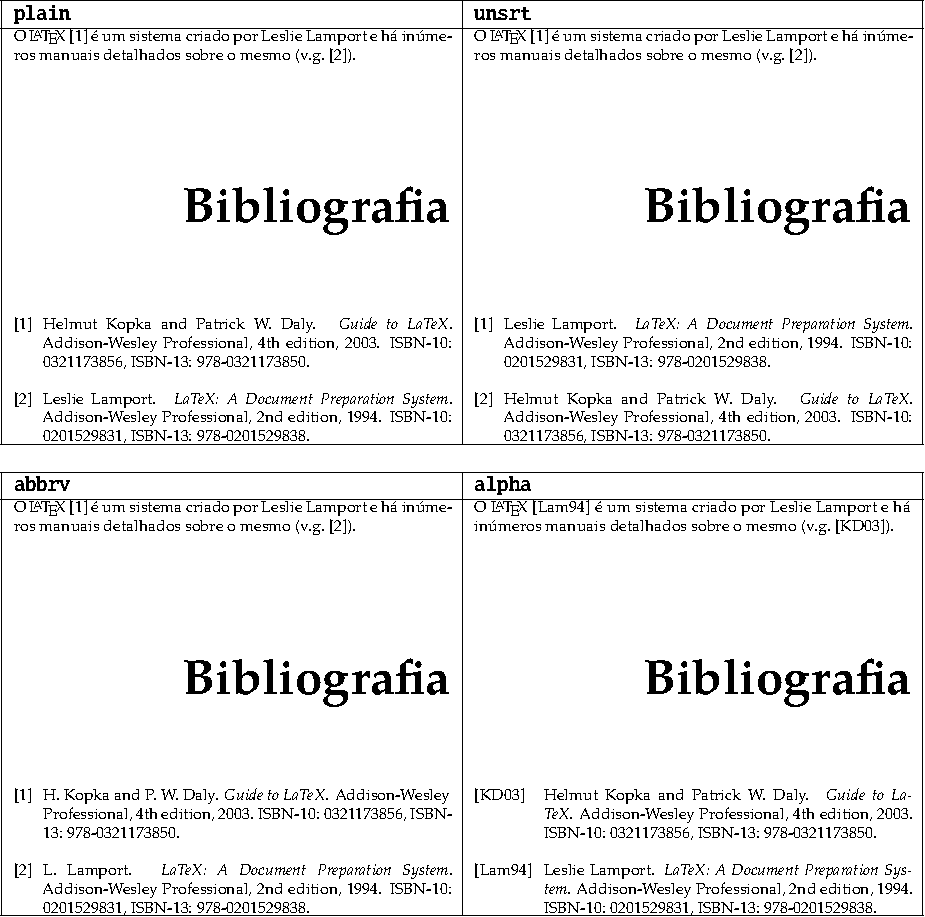
\includegraphics[width=\textwidth]{latex-intro/bib.pdf}
}
\caption{Exemplo do aspeto final da bibliografia consoante o estilo
usado. O indexador de cada registo é exatamente igual ao que
aparecerá ao longo do texto, no local onde for feita a respetiva
referência.}
\label{biblio.Fig}
\end{figure}

\begin{description}
\item \code{plain}: as referências são ordenadas alfabeticamente
     pelo último nome do primeiro autor e são identificadas por um
     número sequencial começando em $1$.
\item \code{unsrt}: as referências são ordenadas pela ordem em que
     são pela primeira vez referenciadas no texto e e são
     identificadas por um número sequencial começando em $1$.
\item \code{abbrv}: similar ao \code{plain} mas as referências
     possuem os nomes e alguns outros campos abreviados.
\item \code{alpha}: similar ao \code{plain} mas as referências
     são identificadas por um acrónimo formado pelas primeiras letras
     do último nome de alguns dos primeiros autores e pelos dois
     algarismos menos significativos do ano de publicação.
\end{description}

Se considerarmos o seguinte trecho de um documento {\LaTeX}:\\

{\small
\inputminted{latex}{latex-intro/bib.tex}
}


\noindent
este texto e a bibliografia produzida tendo em conta estes 4 estilos
apresentados e os registos da \autoref{bib.Fig} estão patentes na
\autoref{biblio.Fig}.

\begin{exercicio}
Edite um ficheiro com registos bibliográficos, coloque lá um de cada
tipo com um número mínimo de atributos (ator, título e ano chegam,
pode inventar). Inclua no seu documento {\LaTeX} os comandos de
inclusão de bibliografia e escolha um estilo. Inclua referência no
seu texto ao registos bibliográficos que criou e gere as respetivas
referências com o comando {\bibtex}. Observe as mensagens de erro
(atributos em falta) reportados pelo {\bibtex} e atribua-os. Proceda
até conseguir ter um documento que cite todas registos
bibliográficos que criou. Altere o estilo de formatação das citações
e observe o resultado.
\end{exercicio}

\chapter{Visão global da geração de documentos {\LaTeX}}
\label{diagram}

Para terminar este documento vamos dar uma visão global do modo como
o {\LaTeX} deve ser usado para produzir um documento complexo. Esta
explicação será ilustrada pela \autoref{fig.bibtex-diagram}.
Os ficheiros fonte
estão a azul, o ficheiro alvo está a preto, os ficheiros verdes são
ficheiros temporários, criados automaticamente, que são fundamentais
para o processo de geração do documento alvo mas que podem em
qualquer altura ser apagados. As setas a vermelho apontam para
resultados de comandos realizados usando como parâmetro o ficheiro no início da
seta. As setas tracejadas a azul representam inclusões de ficheiros
por referência a partir de outros ficheiros, sendo indicado o
comando responsável por essa inclusão.\\



O texto fonte de um documento pode estar repartido por vários
documentos fonte, todos com a extensão \code{.tex}. Na
\autoref{fig.bibtex-diagram} são usados 4, um principal (\code{doc.tex})
e 3 outros incluídos por este usando o comando \verb|\input|.

Para além deste ficheiros, o texto fonte de um documento existe
também ao nível dos ficheiros de registos bibliográficos usados para
retirar referências usadas no documento.  Na
\autoref{fig.bibtex-diagram} são usados 3, os quais são associados ao
documento através do comando \verb|bibliography|.

Resumindo, o documento possui 7 ficheiros fonte, 4 com conteúdos
indiscriminados e 3 com registos {\bibtex}.

A compilação do documento faz-se com o comando \code{pdflatex}
passando como parâmetro o nome base do ficheiro principal do
documento (\code{doc.tex} ou \code{doc}, a extensão pode ser
omitida). Daqui resulta um documento \ac{pdf} (\code{doc.pdf}), que é o
objetivo pretendido, e mais uma série de ficheiros que são um
subproduto da compilação.

Alguns destes ficheiros são meramente informativos, como o
\code{doc.log}, que possui um registo das atividades executadas pelo
comando, ficheiros usados, erros identificados, etc.

\begin{figure}[H]
\centerline{
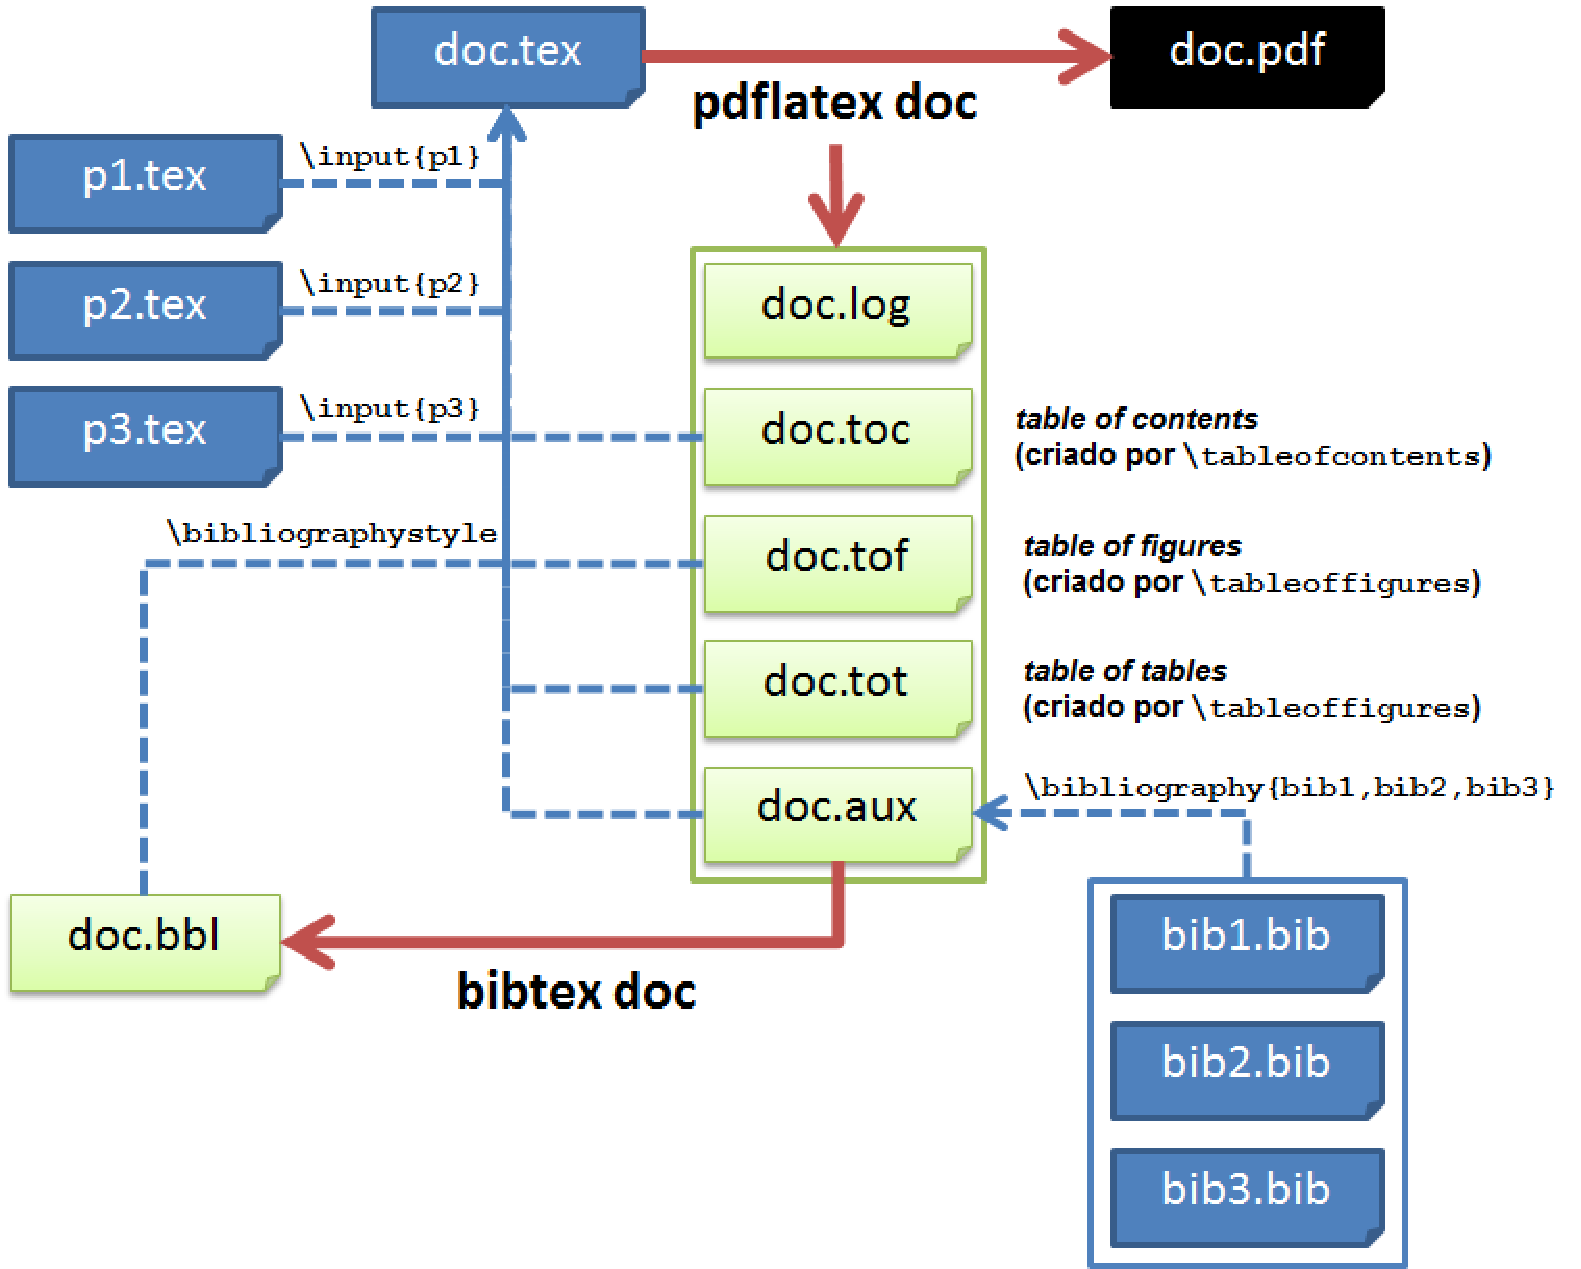
\includegraphics[width=0.8\textwidth]{latex-intro/diagram}
}
\label{fig.bibtex-diagram}
\caption{Ficheiros e comandos envolvidos na geração de um documento
\acs{pdf} a partir de fontes em {\LaTeX} e {\bibtex}}
\end{figure}





Outros são ficheiros que deverão ser usados da próxima vez que o
mesmo comando for executado, e que possuem conteúdos relacionados
com referências. É o caso do índice, que fica guardado no ficheiro
\code{doc.toc} para ser incluído na próxima compilação. O mesmo se
passa com índice de figuras (\code{doc.tof}) e o índice de tabelas
(\code{doc.tot}).

Finalmente, no ficheiro \code{doc.aux} são registadas todas as
atribuições de números a etiquetas, bem como o nome de ficheiros fonte de
registos {\bibtex}. Este ficheiro é usado pelo \code{pdflatex} como
uma fonte de informação auxiliar para obter identificadores
associados a etiquetas. É ainda usado para pelo comando
\code{bibtex} para saber quais são os ficheiros de registos
bibliográficos que devem ser considerados para o ficheiro
\code{doc.tex}.

O comando \code{bibtex} gera um ficheiro de referências
bibliográficas (\code{doc.bbl}) que contém todas as ferências
identificadas pelo \code{pdflatex} quando compilou \code{doc.tex}, e
cuja etiqueta ficou registada em \code{doc.aux}. Estas referências
serão incluídas na próxima compilação de \code{doc.tex}.

É claro, pelo fluxo de dados circular descrito, e apresentado na
\autoref{fig.bibtex-diagram}, que para se gerar um documento \ac{pdf} a
partir de fontes em {\LaTeX} e {\bibtex} é necessário realizar
ciclos de compilação com várias ferramentas até obter um resultado
final completamente correto. O comando \code{pdflatex} dá uma ajuda
neste sentido porque indica, após uma compilação, se é necessário ou
não realizar mais alguma compilação, bem como se há etiquetas
referenciadas mas desconhecidas. Estas indicações ficam igualmente
registadas no ficheiro \code{doc.log}.

\newpage
\chapter{Glossário}

\footnotesize
\SingleSpacing

\begin{multicols}{2}
\begin{acronym}[AAAAAA]

	\acro{h2o}[H2O]{Water}


\end{acronym}
\end{multicols}



\setlength\bibitemsep{8pt}
\printbibliography[heading=bibliography]

\end{document}
